
\subsection{What is \LaTeX?}
LaTeX (pronounced \enquote{Lah-Tech}) is a document preparation system for technical and scientific documents. LaTeX is not a word processor; instead, it encourages authors to focus on content rather than the appearance of their documents\footnote{\url{https://www.latex-project.org/about/}}. 

\begingroup
\captionof{figure}{\LaTeX\ Document example}
\endgroup
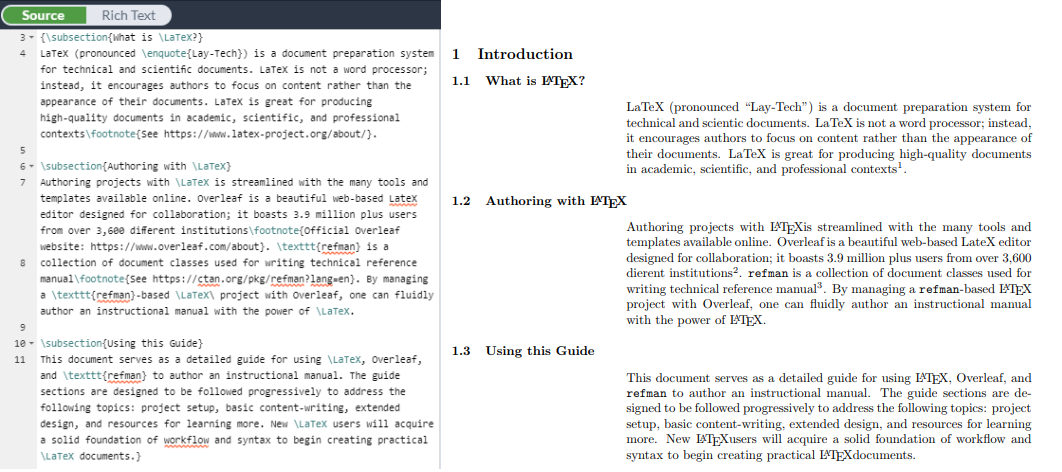
\includegraphics[width=\linewidth]{graphics/IntroSource.png}

\LaTeX is an extension of \TeX, %TODODO

LaTeX is great for producing high-quality technical documents in academic and professional contexts.

\newpage
\subsection{Authoring with \LaTeX}
Authoring projects with \LaTeX\ is streamlined with the many tools and templates available online.
\par
Overleaf is a beautiful web-based \LaTeX editor designed for collaboration; it boasts 3.9 million plus users from over 3,600 different institutions\footnote{\url{https://www.overleaf.com/about}}.
The software has many powerful features including Git integration, change tracking, and rich text editing\footnote{See \url{https://www.overleaf.com/blog/overleaf-v2-launch-announcement}}.

\begingroup
\captionof{figure}{Overleaf feature demonstration}
\endgroup
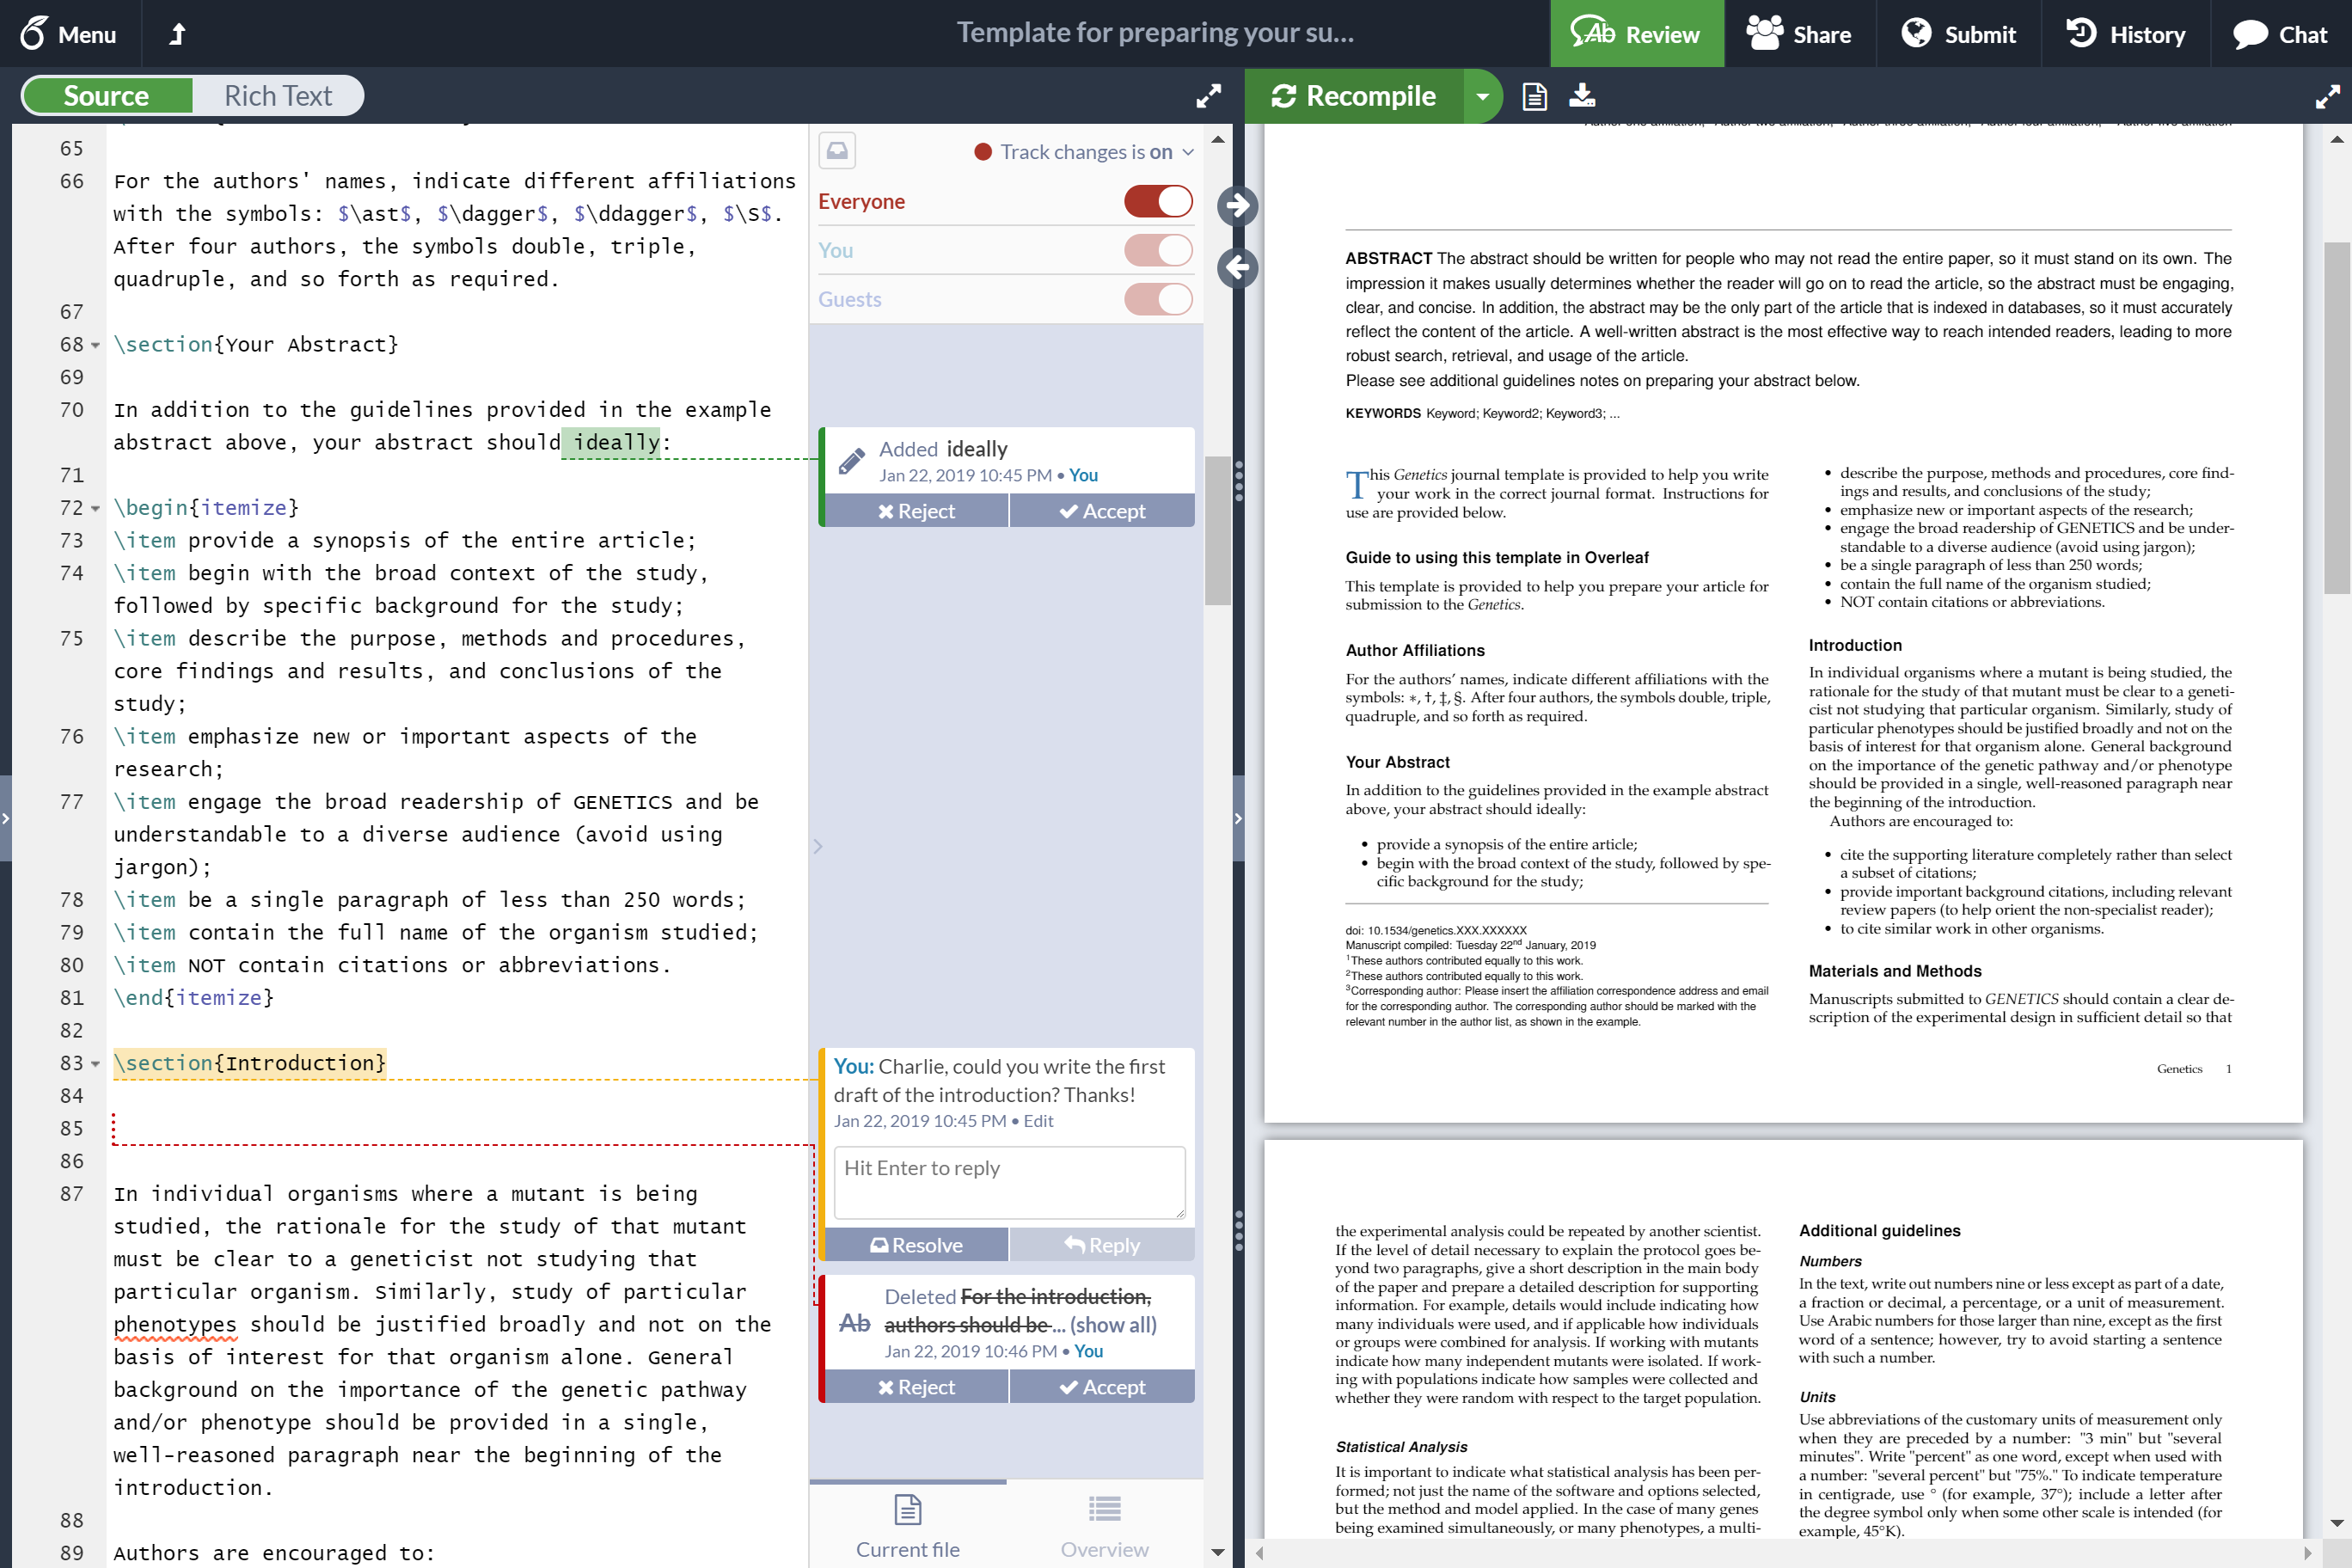
\includegraphics[width=\linewidth]{graphics/OverleafProduct.png}
%https://www.overleaf.com/for/press/resources
\par


\newpage
\texttt{refman} is a collection of document classes used for writing technical reference manuals\footnote{\url{https://ctan.org/pkg/refman?lang=en}}.

\begingroup
\captionof{figure}{Title page of compiled \texttt{refman}}
\endgroup

\includegraphics[width=\linewidth]{graphics/refman.PNG}
%http://ctan.math.illinois.edu/macros/latex/contrib/refman/layout_e.pdf

Overleaf can be used for a \texttt{refman}-based project, allowing authors to create formatted instructional guides with the power of \LaTeX.

\newpage
\subsection{Using this Guide}
This document serves as a detailed guide for using \LaTeX, Overleaf, and \texttt{refman} to author an instructional guide. The guide sections are designed to be followed progressively to address the following topics: project setup, basic content-writing, extended design, and resources for learning more. New \LaTeX\ users will acquire a solid foundation of workflow and syntax to begin creating practical \LaTeX\ documents.